% vim:set et sw=2 ts=4 tw=72:
\chapter{Evaluation}\label{chap:evaluation}

In June 2017, I conducted a study to quantitatively and qualitatively
evaluate the effectiveness of the visualizations and summaries presented
in \tool{} to the DAG-based visualizations found in Gitk and the git
command-line. The study was performed in a controlled environment
running Ubuntu 14.04. Participants were allowed to use Gitk and the git
command-line tools for these tasks, I will refer to both tools as Gitk,
when working with DAG-based visualizations and summarizations. I
considered allowing participants to use any of the free tools for Linux
suggested on the git
website\footnote{\url{https://git-scm.com/download/gui/linux}}, but
after attempting to use them, I found that none were able to operate on
repositories that were as large as the Linux repository. \tool{} was
used for evaluating the \mt{-based} visualizations.

The study has two primary goals; first determining if the DAG-based
visualization is sufficient for conceptual understanding, second
comparing \tool and Gitk to determine which is more capable of providing
users with a summarization of various metrics involved with integrating
a commit into the repository. These were done in two parts of the same
study. They were performed together as a single study for pragmatic
reasons, but could have been done as separate studies.

\section{Methodology}\label{sec:methodology}

This section describes the evaluation, how it was performed, the methods
used to ensure that things were kept consistent between participants,
and setting of the study. The evaluation was performed as a single
study, broken into two parts, using the same 12 participants and same 2
commits. The first part of the evaluation only used Gitk, while the
second part used Gitk and \tool{}. The order that the participants
studied each commit was randomized for each participant, but was kept
consistent through each part of the study. Participants would complete
part one of the study on both commits, the continue with part two, before
answering a few questions about their opinions and experience in an exit
interview. A screencapture with audio was taken for the duration of the
study with each participant. The videos were later analyzed and had the
information extracted into a more usable form.

With some exceptions, three metrics are recorded from each task;
correctness, accuracy, and time taken. Correctness is simply whether the
response was correct. Accuracy is how far from the response was from the
correct answer. An Accuracy of zero indicates that the answer was
correct. Time indicates how long the participant took to respond. Time
is measured from the end of the question to the beginning of the final
response. Since the time measures until the final modification to the
answer, it is possible for times to overlap between tasks if the
participant were to change their response after answering another
question.

Order bias was mitigated throughout the study through the use of
randomization between participants. In both parts, the order that the
participants worked with the commits, tasks, and tools was randomized.
Participant performance, with regard to the recorded performance
metrics, between different size merges, or merges that are merging
different number of commits, is measured in both parts of the study. The
hypothesis being that it is easier to locate commits for and summarize
smaller merges. In the remainder of the \paper{}, merge size refers to
the number of repository events being integrated at a given merge. Two
merge trees are selected from the set of merge trees, and from each of
those, a single commit is selected. The reasoning and method for
selecting the trees and commits is detailed in
Section~\ref{sub:commit_selection}. The order that the commits were
inspected was randomized between participants, and were kept consistent
between parts for each participant. Where applicable, the order that the
tools were used by the participants was randomized between participants.
Details on the randomization of the tasks are outlined with the
methodologies for the specific parts of the study.

Statistical significance testing is performed to verify that the results
are meaningful. An $\alpha = 0.05$ or a $95\%$ confidence level is used.
The Wilcoxon test\cite{Wilcoxon45} is applied between commits to
determine if the size of the \mt effects timing and accuracy. If there
is no statistically significant difference between the distributions of
responses to a task in both commits, then the results of both commits
are aggregated. The McNemar $\chi^2$ test\cite{McNemar1947} with
continuity correction is used to test if there is a difference in the
correctness of responses made by users when using \tool{} versus Gitk.
The Wilcoxon test\cite{Wilcoxon45} and Cliff's effect size\cite{Cliff93}
are applied to the accuracy and timing metrics to determine the
significance of the difference between the results in \tool{} and Gitk.

Prior to starting the study, participants were introduced to the \mt{}
model and the conversion from the DAG to the \mt{}. Two examples of how
the conversion works were given, the examples shown in
Figure~\ref{fig:DAG_to_MergeTree}. Any questions about the model or
conversion were answered at this time. Then participants were introduced
to the tools, Gitk and \tool{}, and could ask questions about either
interface. These introductions usually lasted no more than 10 minutes.

\begin{figure}[htpb]
  \begin{center}
    \begin{tabular}{cc}
      \begin{tikzpicture}[auto, on grid, semithick,
        commit/.style={draw,shape=circle,fill=black}]
        \node[commit] (A) {};
        \node[commit, below right = of A] (1) {};
        \node[commit, below = of 1] (2) {};
        \node[commit, below = of 2] (3) {};
        \node[commit, below left = of 3] (I) {};

        \node[left = 0.5cm of A] {A};
        \node[right = 0.5cm of 1] {1};
        \node[right = 0.5cm of 2] {2};
        \node[right = 0.5cm of 3] {3};
        \node[left = 1.0cm of I] {Initial};

        \draw (A) edge[-stealth] (I) edge[-stealth] (1)
              (1) edge[-stealth] (2)
              (2) edge[-stealth] (3)
              (3) edge[-stealth] (I);
    \end{tikzpicture}
    &
    \begin{tikzpicture}[auto, on grid, semithick,
      root/.style={draw, circle, minimum size=0.8cm},
      leaf/.style={draw, circle, minimum size=0.8cm}]
      \node[root] {A}
      child {node[leaf] {1}}
      child {node[leaf] {2}}
      child {node[leaf] {3}};
    \end{tikzpicture}
    \\\midrule
    \begin{tikzpicture}[auto, on grid, semithick,
        commit/.style={draw,shape=circle,fill=black}]

        \node[commit] (A){};
        \node[commit, below right = of A] (1) {};
        \node[commit, below = of 1] (B) {};
        \node[commit, below = of B] (2) {};
        \node[commit, below = of 2] (3) {};
        \node[commit, below right = of B] (4) {};
        \node[commit, below left = of 3] (I) {};

        \node[left = 0.5cm of A] {A};
        \node[right = 0.5cm of 1] {1};
        \node[left = 0.45cm of B] {B};
        \node[left = 0.45cm of 2] {2};
        \node[left=0.45cm of 3]{3};
        \node[right=0.5cm of 4] {4};
        \node[left=1.0cm of I] {Initial};

        \draw (A) edge[-stealth] (I) edge[-stealth] (1)
              (1) edge[-stealth] (B)
              (B) edge[-stealth] (2) edge[-stealth] (4)
              (2) edge[-stealth] (3)
              (4) edge[-stealth] (3)
              (3) edge[-stealth] (I);
    \end{tikzpicture}
    &
    \begin{tikzpicture}[auto, on grid, semithick,
      every node/.style={draw, circle, minimum size=0.8cm}]
      \node {A}
      child {node {1}}
      child {node {B} child {node {4}}}
      child {node {2}}
      child {node {3}};
    \end{tikzpicture}
    \end{tabular}
  \end{center}
  \caption{Two examples of DAG to \mt{} conversions used in explanation
  during evaluation}
\label{fig:DAG_to_MergeTree}
\end{figure}

Following the introduction, participants worked through the tasks in the
conceptual portion of the study and comparative summarization portion of
the study. Details for the conceptual study and summarization study are
in Section~\ref{sub:conceptual_study}, and
Section~\ref{sub:summarization_study} , respectively. The study
concluded with participant opinions and a short exit interview to
collect information about the experience of the participants with
version control software. Details of which are provided in
Section~\ref{sub:user_opinions_and_exit_interview}.

\subsection{Commit Selection}\label{sub:commit_selection}

Two commits are used in both the conceptual study and summarization
study, with the goal of determining how well the DAG and \mt{}
visualizations scale between merges integrating varying numbers of
commits. The order that the two commits are presented to each
participant is randomized. I analyzed 15096 \mt{s} from the
database that were candidates for the study, from April 16th 2005 to
October 14th 2014, corresponding to Linux releases 2.6.12-rc3 to
3.17-rc1. A \mt{} could only be selected if it was not a foxtrot,
and had correctly been identified. 25\% of the trees contain at most a
single repository event, not including the root, while 50\% of the trees
contain at most seven nodes. 75\% of the trees contain at least 51
nodes, and the largest tree contains 7217 nodes. 8031 trees contained at
least seven nodes, of these only 593 contained at least a single
internal merge node. Trivially, trees with a single node cannot have any
internal merge nodes. Of the 624 trees with seven non-root node, only
135 contained at least one inner node. Using this information, I chose a
random tree from the 2008 trees in the first quartile, which merges a
single commit into the master branch. These trees are trivial, but
appear frequently in the repository. The second tree was chosen randomly
from trees in the second quartile. These trees contain seven nodes, and
to increase the complexity of the tree, I required that the tree contain
at least one internal merge node.

Once the trees were selected, I had to select a commit from the tree.
Selecting a commit from the small tree was trivial, there was only a
single node to choose. From the medium-sized tree, I used a script to
select a commit randomly. The commits selected from the small tree and
medium tree were \emph{a3c1239eb59c0a907f8be5587d42e950f44543f8} and
\emph{cdbdd1676a5379f1d5cbd4d476f5e349f445befe} respectively. Commit 1,
the commit from the small tree is visualized in
Figure~\ref{fig:commit_1_visualization}, showing the DAG visualization
by Gitk and \rt{} tree visualization in Linvis. The same is
shown for commit 2 in Figure~\ref{fig:commit_2_visualization}.

\begin{figure}[htpb]
  \centering
  \begin{tabular}{cc}
    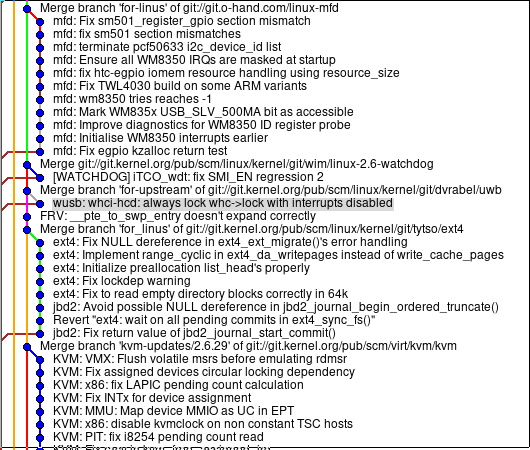
\includegraphics[height=4.5cm]{Figures/evaluation/commit1_gitk.png} &
    
\includegraphics[height=4.5cm]{Figures/evaluation/commit1_linvis.pdf}
  \end{tabular}
  \caption{The visualizations of commit 1 by Gitk and Linvis
    respectively.}
  \label{fig:commit_1_visualization}
\end{figure}

\begin{figure}[htpb]
  \centering
  \begin{tabular}{cc}
    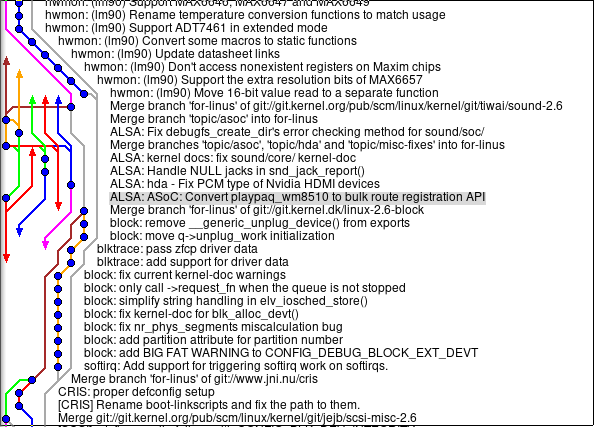
\includegraphics[height=4.5cm]{Figures/evaluation/commit2_gitk.png} &
    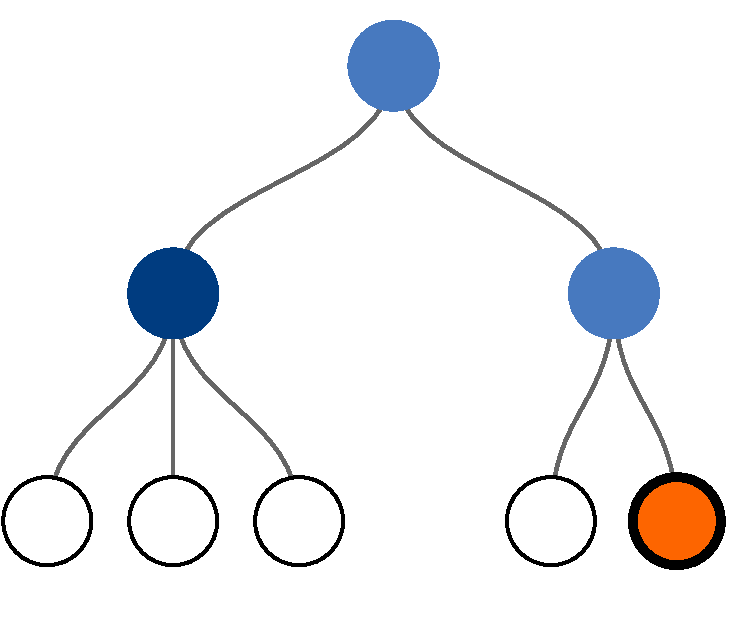
\includegraphics[height=4.5cm]{Figures/evaluation/commit2_linvis.pdf}
  \end{tabular}
  \caption{The visualizations of commit 2 by Gitk and Linvis
    respectively.}
  \label{fig:commit_2_visualization}
\end{figure}

\subsection{Part 1: Conceptual Study}\label{sub:conceptual_study}

The conceptual portion of the study verifies our initial assumption,
that the DAG visualization is unable to provide people with a conceptual
understanding of the events in a repository. Participants in the study
are asked to perform tasks that are related to understanding how a
commit is integrated. The tasks for this part of the study are outlined
in Table~\ref{tab:conceptual_tasks}.

\begin{table*}[htpb]
  \centering
  \caption{Conceptual Tasks}
  \label{tab:conceptual_tasks}
  \begin{tabulary}{0.9\textwidth}{LL}
    \toprule
    Task & Description\\
    \midrule
    T1 & Draw a diagram showing how this commit was merged into the master branch, along with any other related commits\\
    T2 & How many individual commits are related to this commit?\\
    T3 & How many merges are involved with merging this commit into the master branch?\\
    \bottomrule
  \end{tabulary}
\end{table*}

Task 1 asks participants to draw a diagram showing the shortest path for
a commit to be merged, including any commits that are related to it, or
are necessary for the integration. Participants were given 10 minutes to
draw the diagram. The correct answer should look something like the
\mt{} for that commit. The drawing from Task 1 is then referred to
in Task 2 and 3. Building on the conceptual understanding built in task
1, task 2 and 3 ask the participant to determine how many commits are
related, and how many merges. The order that task 2 and 3 are presented
to participants is randomized between participants, to remove order
bias, although it shouldn't matter as both questions are designed to
build off of task 1 and the conceptual understanding constructed  from
analyzing the DAG visualization of that commit for 10 minutes. These
questions enable us to find issues when users are comprehending the DAG
visualizations.

The diagrams drawn by the participants in the first task help provide
insight about how the participants are interpreting the DAG. I looked
for patterns in the drawings to see if common issues arose, providing
qualitative information about issues in comprehension. The results from
task 2 and 3 are numerical results, the number of commits that are
related, and the number of merges. These numbers are directly comparable
with the correct numbers.

\subsection{Part 2: Summarization Study}\label{sub:summarization_study}

The summarization portion of the study compares the visualization and
summarization capabilities of \tool{} and Gitk to determine if the
visualization of the \mt{} is capable of providing a better
understanding of the events in repository, specifically answering
RQ\ref{rq:RQ2} and RQ\ref{rq:RQ3}. This portion of the study requires the
participants to switch between both Use-Case 1 and Use-Case 2
strategies. The participants are provided an commit, since their goal is
to summarize information about the entire \mt{}, they must navigate
to the root node, making use of features for Use-Case 1. Once they are
at the root, the participant must be able to summarize information about
the authors, files, and modules. The tasks are outline in
Table~\ref{tab:summarization_tasks}.

\begin{table}[htpb]
  \centering
  \caption{Summarization Tasks}
  \label{tab:summarization_tasks}
  \begin{tabular}{lll}
    \toprule
    Task Set   & Task & Description\\\midrule
    Merge      & T4   & What is the series of merges involved with merging this
    commit?\\
               & T5   & What other commits are merged?\\
    Authorship & T6   & How many authors are involved?\\
               & T7   & Who contributed the most changes?\\
    Files      & T8   & How many files were modified?\\
               & T9   & Which file had the most changes?\\
    Modules    & T10  & Which modules does this \mt involve?\\
    \bottomrule
  \end{tabular}
\end{table}

For each task, where specified, four statistical tests are applied. The
first test determines if the results from the two commits are from the
same distribution. If they are, it indicates that the results can be
aggregated, otherwise, the results must be analyzed for each commit
separately. The three other tests measure the difference in correctness,
accuracy, and time between the results for \tool{} and Gitk. The null
hypothesis for the difference between the commits is that there is no
difference in the performance metrics between the commits. For the
correctness metric, the null hypothesis is that \tool{} does not effect
the correctness of the participants. For the accuracy metric, the null
hypothesis is that there is no difference in accuracy between the
results drawn from \tool{} and from Gitk. For the timing metric, the null
hypothesis is that there is no difference in timing between the time
taken to draw a result from \tool{} and Gitk.

The tasks are split into four task sets, based on the type of
information that the task is investigating. The \emph{Merge} tasks set
focuses on detailed information about the topology of the merge itself,
looking at the specific merges and commits involved in the integration.
Task T4 asks for the specific merges that merge the commit into the
master branch. These must be the correct merges, and must be in the
correct order. I use the edit distance between the response and the
correct answer as a measure of how correct the response is. Adding new
merges, removing extraneous merges, replacing merges, and swapping the
order of merges are of unit cost. An edit distance of 0 indicates a
correct answer. Task T5 asks for the other commits that are integrated
with this commit. Again, I use an edit distance-like metric to evaluate
the response. Order doesn't matter, but the correct commits must be
indicated in the response. Adding commits, replacing commits, and
removing commits are of unit cost.

The \emph{authorship} task set involves finding information about the
authors involved in the merge. Task T6 asks for the number of authors
involved in the merge. These are authors of commits, not merges, as
merges in the kernel repository do not include code, and are used for
creating logical separation in commits. The accuracy is measured as the
absolute difference between the response and the correct answer. Task T7
asks participants to identify the person who was responsible for
contributing the most in the merge. While it is possible that two
authors could have contributed the same number of changes, in the merges
for both commits, there is an identifiable author who contributed the
most. The answer to this task can either be correct or incorrect, so
accuracy is not recorded for this task.

The \emph{files} task set involves finding information about specific
files being merged. Task T8 asks the participant to identify how many
files are modified in a merge. Like task T6, the response to task T8 is
a single number, so the accuracy is measured as the absolute difference
between the response and the correct answer. Task T9 asks the
participants to identify which files had the most lines modified in
the merge. While this is similar to task T7, the files in the tree
associated with commit 1 had the same number of changes. For this
reason, I use the edit distance between the response and the correct
answer, with addition, removal, and replacement of unit cost.

The \emph{modules} task set only contains a single task, and involves
determining the modules involved in a merge. Modules, or subsystems,
refer to the component of the kernel that is being modified by a commit.
This is not a property that is inherent to git repositories in general,
but a property I noticed in the repository of the Linux kernel. Commit
summaries are prefaced with the module, followed by a colon. For example
the log summary \textit{``ALSA: kernel docs: fix sound/core/
  kernel-doc''} is in the \textit{``ALSA''} module.

The order that the task sets are performed is randomized between
participants, and the order that the tasks within a task set are
performed is randomized as well. This keeps related tasks together,
while still mitigating some of the order bias.

\subsection{User Opinions and Exit Interview}
\label{sub:user_opinions_and_exit_interview}

The goal in this part of the study is to expose issues in the underlying
assumptions made while writing \tool{}. Two questions were asked in this
part of the study, outlined in Table~\ref{tab:opinion_questions}. This
portion of the study gives the participants to voice their opinions and
observations that may not have been recorded or captured by the rest of
the study.

\begin{table}[htpb]
  \centering
  \caption{User Opinion Questions}
  \label{tab:opinion_questions}
  \begin{tabulary}{0.9\textwidth}{LL}
    \toprule
    Question & Description\\
    \midrule
    Q1 & Given these tasks again, which tool would you prefer?\\
    Q2 & Which aspects of each tool did you like and why?\\
    \bottomrule
  \end{tabulary}
\end{table}

Question Q1 allows users to express their opinions on tool preference
for merge-summarization tasks. Neither \tool{} nor Gitk are perfect,
participants may have complaints or aspects of each tool that they
preferred, or aspects that assisted them in understanding the events in
the repository. Question Q2 is meant to address this.

The exit interview is designed with the goal of collecting some
information about our participants, and their experience with version
control software and git. Three questions were asked in the exit
interview portion of the study;

\begin{itemize}
  \item For how long have you used git?
  \item For what kind of projects have you used git?
  \item How many commits, files, and collaborators were involved with
    the largest repository you have worked with?
\end{itemize}

\section{Participant Profile}\label{sec:participant_profile}

The study was conducted with 12 participants, all of whom were masters,
PhD, or post-doc researchers in the field of software engineering. The
participants had between 6 months and 10 years experience with git, with
the median being 3.5 years. Most participants had additional experience
with SVN and CVS.\@ One of the participants in the study worked as a
release engineer, studying merge practices to determine the best way to
merge branches while minimizing the number of merge conflicts in SVN
repositories. The participants worked with repositories ranging from
around 10 commits up to 38000 commits, with the median being 350
commits. Two of the participants had never collaborated with anyone in a
repository, while the rest had some experience with repositories being
modified by multiple people, with the most being 219. The median number
of collaborators was four. Participants had most experience with
personal and academic repositories. Three of the twelve participants had
experience with professional repositories.

All participants have had at least some experience with version control,
branching in repositories, and git. The participants are from the same
lab, and each participant worked with both tools in the study, thus,
keeping the sample populations identical for both tools, with some
variation between participants in experience with repositories.

\section{Results}
\label{sec:results}

This section presents the results from the user study. The results for
the conceptual tasks are presented in
Section~\ref{sub:conceptual_results}, for the summarization tasks in
Section~\ref{sub:summarization_results}, and the user opinions in
Section~\ref{sub:user_opinions_results}.

\subsection{Conceptual Study Results}
\label{sub:conceptual_results}

Investigating the drawings made in response to task T1, none of the
results from this task are correct. The diagrams for commit 1 tend to
resemble a linked list, showing all of the merges along the master
branch. The participants would generally continue traversing the master
branch using either the first parent or the child links in the Gitk
interface, or simply following the branch in the visualization, until
they either hit the branch tag \verb|2.6.29-rc6|, or indicated that it
was every merge along the master branch, or stopped at a seemingly
arbitrary merge. An example of a diagram drawn by one participant is
shown in Figure~\ref{fig:commit_1_fig}. This drawing follows the DAG
backward, working from the commit, through the branch point, and
traversing the DAG toward the initial commit. In another case, the
participant was able to produce the correct drawing using the git
command line tools, but then looked at the DAG visualization in Gitk and
continued to draw a linked list, following the merges along the master
branch toward the HEAD node.

\begin{figure}[htpb]
  \centering

  \begin{tikzpicture}[commit/.style={ellipse, text=black, draw=black}]
    \node[commit] (a) {11df};
    \node[commit, right = of a] (b) {a3c};
    \node[commit, right = of b] (c) {d2f8};
    \node[commit, right = of c] (d) {b51e};
    \node[commit, right = of d] (e) {fb5};
    \node[commit, right = of e] (f) {37b};

    \draw (a) edge[-stealth] (b)
          (b) edge[-stealth] (c)
          (c) edge[-stealth] (d)
          (d) edge[-stealth] (e)
          (e) edge[-stealth] (f);
  \end{tikzpicture}

  \caption{Example of a diagram drawn for the integration of commit 1}
  \label{fig:commit_1_fig}
\end{figure}

This indicates difficulties identifying the master branch in the
visualization. Furthermore, the commit date should provide some
indication on which direction the commits are being merged in, some
participants did not understand this from the Gitk interface. This could
be confusion looking at the interface, or in the terminology surrounding
the parent-child relationship.

The resulting diagrams for commit 2 do not show any consistent patterns
among participants. Many diagrams do not show the shortest paths from a
commit to the master branch. Some participants were able to identify the
master branch in this case. These participants had experience with SVN
repositories, and were accustomed to the master branch being the first
branch in the graph. In the visualization of the DAG for commit 2, the
master branch returns to the first position in the graph, which some
participants mentioned meant that it should be the master branch. In
this case, they are correct in that the first line in the visualizations
is the master branch in this case, but the reasoning is not correct. The
first branch is not necessarily the master branch, as is the case with
the results from Commit 1, where the master branch is the third line.
Furthermore, the line indicating the master branch creates a visual cage
around the repository events in question, which may have assisted with
finding the correct commits.

\evan{Since the part about the visual cage is speculation, should that
  be moved to discussion?}

With some participants, there was confusion about the direction of the
parent-child relationship. In most data structures, the parents point
toward the node of interest. In this case, the parents point toward the
branch point, which is in the opposite direction of the merge, so the
participant would actually need to follow the child to get to the merge
point.

One participant was able to identify the path to the master branch, but
no participants were able to identify the commits that were necessary
for integrating the given commit into the master branch. The diagram
drawn is shown in Figure~\ref{fig:commit_2_fig}, which shows a possible
path for the commit to pass through on the way to the master branch.
While it isn't the shortest path, it is a possible path. In the diagram,
$M_3$ is the merge into the master branch, and $start$ the commit that
is being queried. The diagram includes one other commit that is being
merged, but there are three additional commits that were not included.
In the \mt{} representation, the starting commit and the $ALSA\ Fix$
commit are both merged into $M_2$, while three others are merged into
$M_1$. $M_1$ and $M_2$ are merged directly into the master branch at
$M_3$. In the other cases, the diagrams had little resemblance of the
events occurring in the repository. Some diagrams appeared to be
constructed from random commits, others did not conform to the tree
structure as what would be constructed from using shortest paths.

\begin{figure}[htpb]
  \centering
  \begin{tikzpicture}[commit/.style={ellipse, draw=black, text=black}]
    \node[commit] (a) {$M_3$};
    \node[commit, below = of a] (b) {$M_2$};
    \node[commit, below right = of b] (c) {$ALSA\ Fix$};
    \node[commit, below left = of b] (d) {$M_1$};
    \node[commit, below = of d] (e) {$start$};

    \draw (e) edge (d)
          (d) edge (b)
          (c) edge (b)
          (b) edge (a);
  \end{tikzpicture}
  \caption{Example of a diagram drawn for the integration of commit 2.
    This diagram is the closest to being a possible representation of
    the events in the repository, but miss the other commits involved.}
  \label{fig:commit_2_fig}
\end{figure}

The participants were better able to determine the number of merges a
commit passed through, and the number of commits being merged in the
larger merge tree, as seen in Table~\ref{tab:conceptual_results}. The
results reported in this table are in number of commits for Task T2, and
the number of merges for task T3. Commit 1, which was merged directly
without any other related commits, was said to have a median of 6
related commits. The median number of merges was said to be between 6
and 7 merges. The correct answer should have been 1, the integrating
merge. There was more disagreement when determining the number of
commits, in both commits. Interestingly, there was more variance in the
answers on the smaller merge tree. The variance in the answers for
determining the number of merges was consistent between both trees.

\begin{table}[htpb]
  \centering
  \caption{Variance and Difference between correct answers and user
    responses in conceptual tasks in tasks T2 and T3}
  \label{tab:conceptual_results}
  \begin{tabular}{ccccc}
    \toprule
    Task & Commit   & Median Difference & Average Difference & Answer Variance\\\midrule
    T2   & Commit 1 & 5                 & 20                 & 803.43\\
    T3   & Commit 1 & 5.5               & 7.8                & 56.18\\
    T2   & Commit 2 & 2                 & 6.22               & 120.19\\
    T3   & Commit 2 & 1                 & 3.67               & 48.5\\
    \bottomrule
  \end{tabular}
\end{table}

Participants generally took longer to respond to questions about the
larger merge tree, and the time taken was far more variable. The timing
results are listed in Table~\ref{tab:conceptual_time_results}. When
interpreting these results, it must be noted that participants had spent
10 minutes working with the merge tree that they were summarizing prior
to answering the questions. These times do not indicate the time to read
the DAG, but the time taken to understand the conceptual image of the
events in the DAG. It took the participants longest to determine the
number of commits in both cases, but it took far longer in the case of
commit 2, taking over half a minute.

\begin{table}[htpb]
  \centering
  \caption{Timing Results from the conceptual tasks T2 and T3}
  \label{tab:conceptual_time_results}
  \begin{tabular}{ccccr}
    \toprule
    Task & Commit   & Median Time (s) & Average Time (s) & Time Variance (s)\\\midrule
    T2   & Commit 1 & 9               & 53.45            & 6382\\
    T3   & Commit 1 & 8               & 26.64            & 921\\
    T2   & Commit 2 & 35              & 114.45           & 58769\\
    T3   & Commit 2 & 15              & 71.36            & 32324\\
    \bottomrule
  \end{tabular}
\end{table}

Users were able to more closely estimate the number of commits and
merges in the larger tree, but generally took longer than the smaller
tree. The tree with a single node resulted in more variability in the
estimate of number of commits.

\subsection{Summarization Study Results}
\label{sub:summarization_results}

Merge size does not affect \textbf{correctness}; however, task T5,
finding the other commits being integrated, and task T9, determining
which file had the most changes, are very close to the $p$-value
threshold. The results of the Wilcoxon test on correctness are shown
Table~\ref{tab:cross_commit_correctness}. Most of the $p$-values are
reasonable far from the threshold of 0.05; however, in tasks T5 and T9,
the $p$-value is within 0.01 of the threshold. Further investigation
reveals that the differences in the distributions stem from the number
of participants who were incorrect when using \tool{}. Inspecting the
results from task T5, in Figure~\ref{fig:T5_correctness}, no
participants provided an incorrect response using \tool{} in the small
merge, but four participants provided an incorrect response when using
\tool{} for the larger merge. Similarly, the number of incorrect
responses increased going from the small merge to the large merge with
Gitk. The split results are similar in task T9.

\begin{table}[htpb]
  \centering
  \caption{Effect of merge size on correctness}
  \label{tab:cross_commit_correctness}
  \begin{tabular}{clr}
    \toprule
    Task & $p$-value & Conclusion\\\midrule
    T4   & 0.16      & Do not reject $H_0$\\
    T5   & 0.05      & Do not reject $H_0$\\
    T6   & 0.11      & Do not reject $H_0$\\
    T7   & 0.08      & Do not reject $H_0$\\
    T8   & 0.13      & Do not reject $H_0$\\
    T9   & 0.06      & Do not reject $H_0$\\
    T10  & 0.45      & Do not reject $H_0$\\
    \bottomrule
  \end{tabular}
\end{table}


\begin{figure}[htpb]
  \centering
  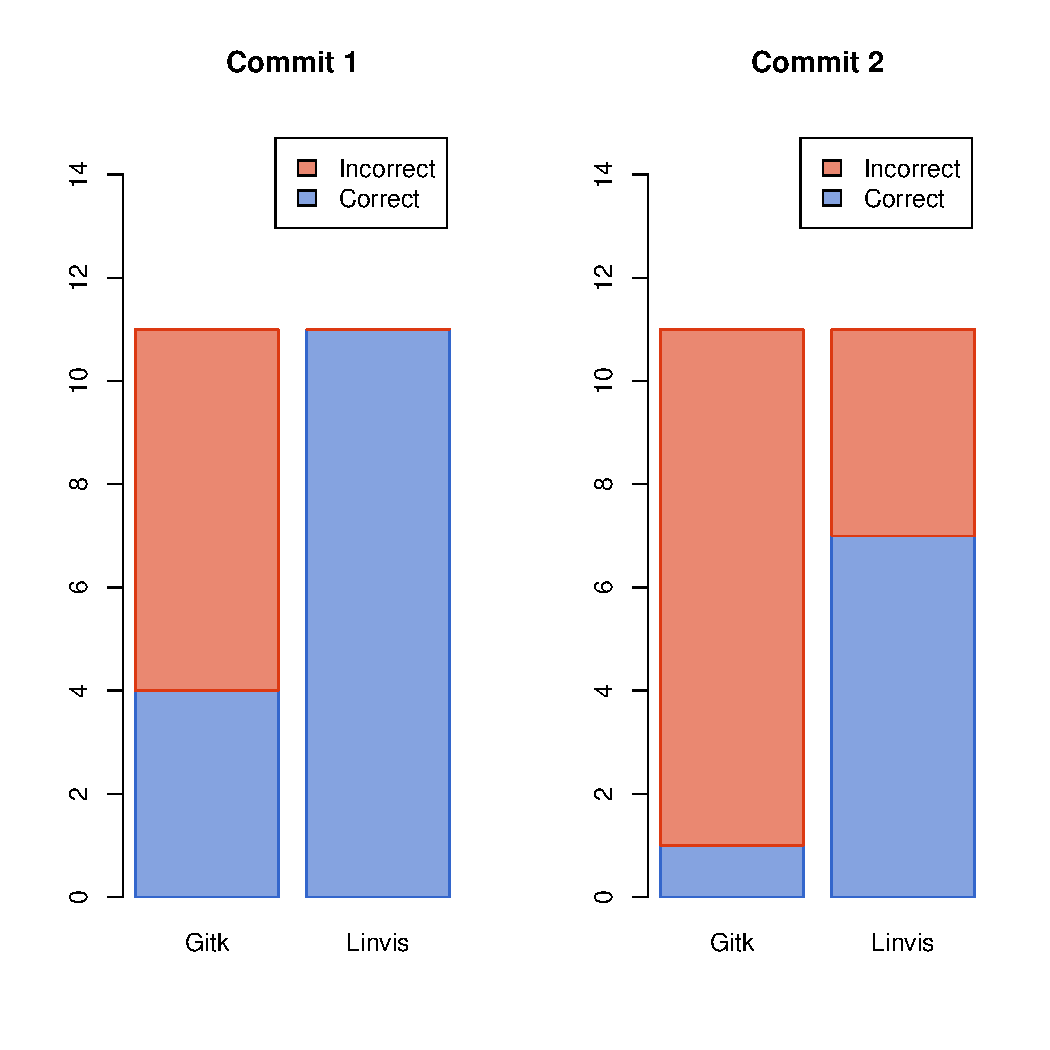
\includegraphics[width=0.4\linewidth]{Figures/evaluation/correctness/5.pdf}
  \caption{Difference between commits in the correctness of responses to task T5.}
  \label{fig:T5_correctness}
\end{figure}


\begin{figure}[htpb]
  \centering
  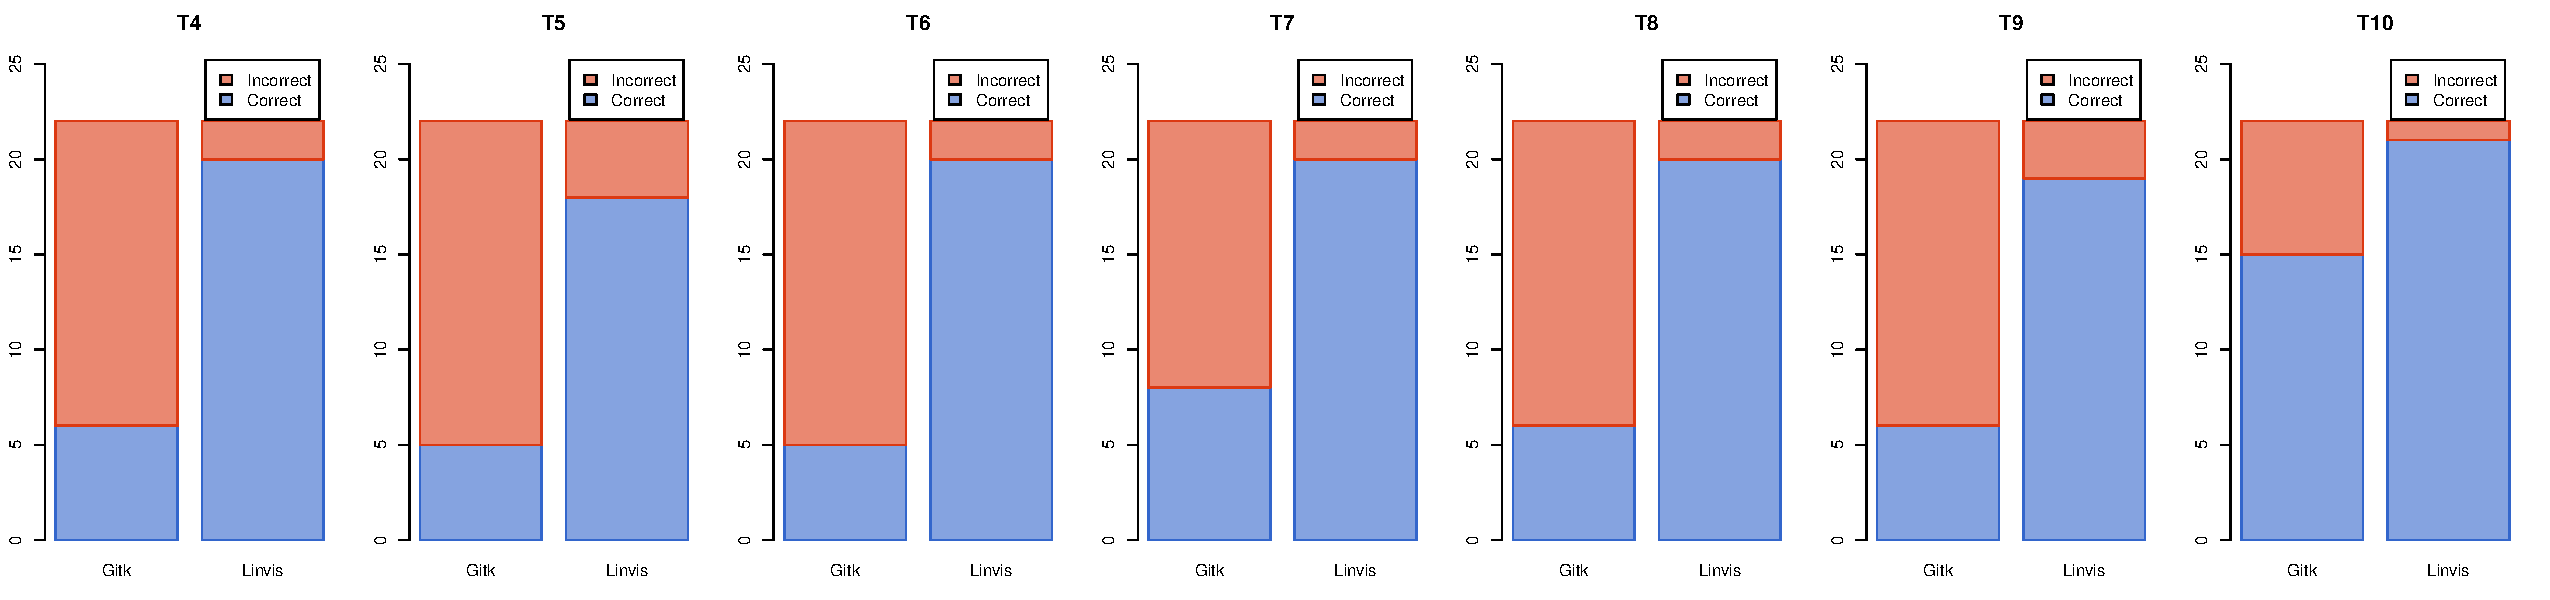
\includegraphics[width=1.0\linewidth]{Figures/evaluation/correctness.pdf}
  \caption{Aggregated Correctness of the summarization results}
  \label{fig:agg_correctness}
\end{figure}

The results do not indicate that there is a difference in the
distributions between the merge sizes, although one might arise with
tasks T5 and T9 with more samples, the results for both merges are
combined. The McNemar test is applied to determine if \tool{} has an
effect on the correctness. The results of the McNemar test are presented
in Table~\ref{tab:mcnemar_test_results}. For each task, except for task
T10, determining which modules are involved in a merge, \tool{} has an
effect on the results. Inspecting the results in
Figure~\ref{fig:agg_correctness} shows that \tool{} effects results in a
positive way, helping users to correctly identify properties about the
merge. In task T10, it is also evident that participants were able to
determine the module involved using both tools.

\begin{table}[htpb]
  \centering
  \caption{Aggregated Correctness Results comparing \tool{} and Gitk}
  \label{tab:mcnemar_test_results}
  \begin{tabular}{crrc}
    \toprule
    Task & $\chi^2$ & $p$-value & Conclusion\\\midrule
    T4   & 12.07    & 0.0005    & Reject $H_0$\\
    T5   & 11.08    & 0.0007    & Reject $H_0$\\
    T6   & 13.07    & 0.0003    & Reject $H_0$\\
    T7   & 10.08    & 0.0015    & Reject $H_0$\\
    T8   & 12.07    & 0.0005    & Reject $H_0$\\
    T9   & 11.08    & 0.0009    & Reject $H_0$\\
    T10  & 3.13     & 0.0771    & Do not reject $H_0$\\
    \bottomrule
  \end{tabular}
\end{table}

Merge size does not affect \textbf{accuracy} in any of the tasks, as
seen in Table~\ref{tab:cross_commit_accuracy}. The results in task T9
are very close to the threshold. Inspecting the distributions in
Figure~\ref{fig:cross_commit_T9_accuracy}, the distribution for \tool{}
appears to be different in the two commits. In commit 1, there is no
variance, the entire distribution is at 0 files from the correct answer.
In commit 2, the 3rd quartile spans from 0 files up to 1 file from the
correct answer, and the fourth quartile, from 1 file to 2 files. This is
consistent with the results found for correctness, although, unlike with
correctness where task T5 showed more difference between merge sizes,
task T9 shows more difference between merge sizes with accuracy. This
indicates that those who were incorrect, were also further from the
correct answer in the larger merge than the small merge in T9 than in
task T5.

\begin{table}[htpb]
  \centering
  \caption{Effect of merge size on accuracy}
  \label{tab:cross_commit_accuracy}
  \begin{tabular}{clr}
    \toprule
    Task & $p$-value & Conclusion\\\midrule
    T4   & 0.97      & Do not reject $H_0$\\
    T5   & 0.08      & Do not reject $H_0$\\
    T6   & 0.21      & Do not reject $H_0$\\
    T8   & 0.13      & Do not reject $H_0$\\
    T9   & 0.06      & Do not reject $H_0$\\
    T10  & 0.22      & Do not reject $H_0$\\
    \bottomrule
  \end{tabular}
\end{table}

\begin{figure}[htpb]
  \centering
  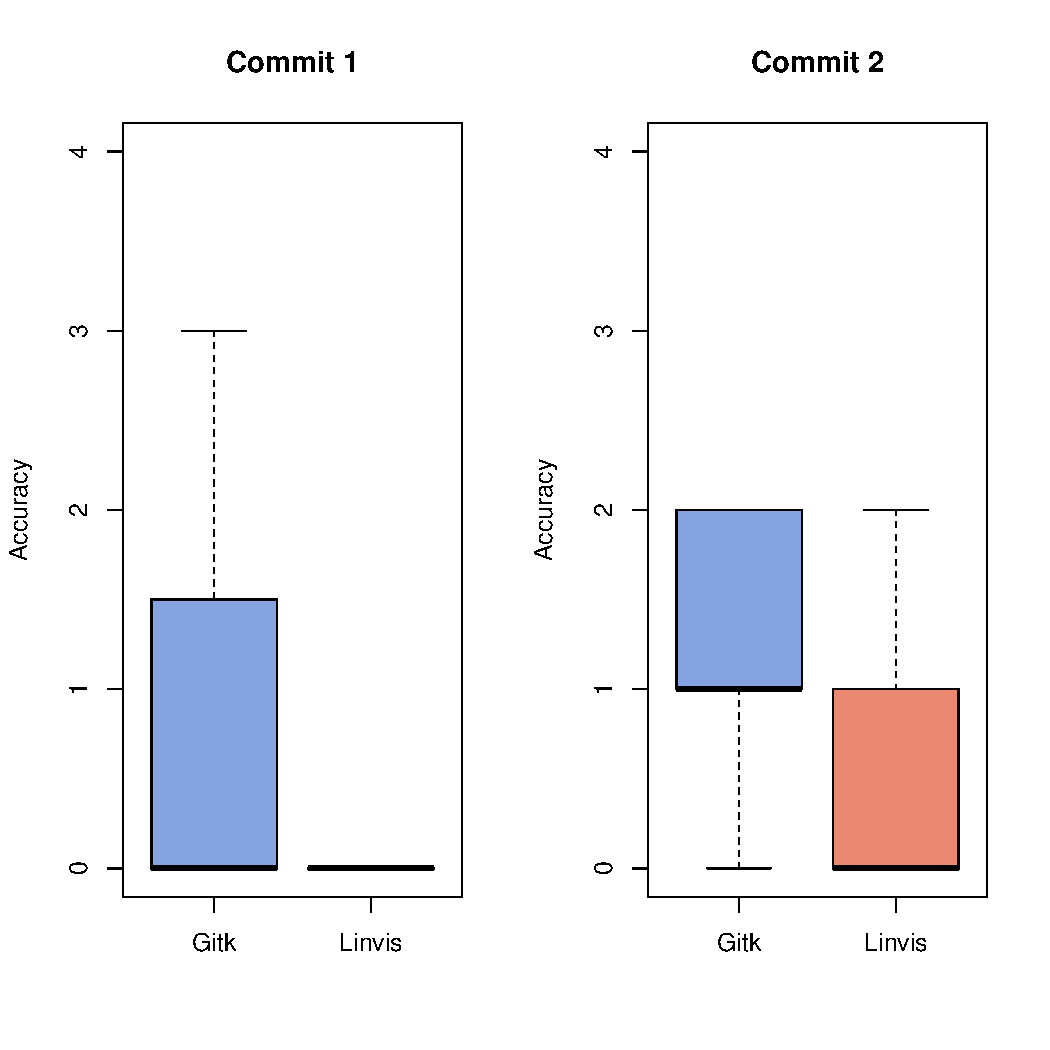
\includegraphics[height=4.5cm]{Figures/evaluation/accuracy/9.pdf}
  \caption{Difference in accuracies in responses to task T9 between Commit 1 and Commit 2.}
  \label{fig:cross_commit_T9_accuracy}
\end{figure}

The results do not indicate a difference in the accuracy distributions
between commits. Again, this could change in tasks T5 and T9 with a
larger sample size. The results for both merges are combined. The
Wilcoxon test and Cliff's Delta effect size are applied to each to
determine if there is a difference in the accuracies of responses to the
tasks between tools. The results of the tests are presented in
Table~\ref{tab:accuracy_results}. In all cases, there is a difference
in accuracies between when the participants use \tool{} versus Gitk. In
all cases except for task T9, which files had the most changes, and T10,
which modules were involved, there was a large effect in favour of
\tool{}. In task T9, there was a medium effect, and T10, a small effect.
Looking at the results depicted in Figure~\ref{fig:agg_accuracy}, this
makes sense. The variance in the accuracies of responses of Gitk is much
smaller in tasks T9 and T10 than in the other tasks, furthermore, the
median is much closer to zero than in the other tasks. In task T10, only
the third and fourth quartiles are beyond 0, which indicates that
participants were generally correct when using Gitk to determine the
module. This is also consistent with the results measuring the
correctness.

\begin{table}[htpb]
  \centering
  \caption{Aggregated Accuracy results, including the Wilcoxon
    $p$-values and Cliff's Delta Effect size}
  \label{tab:accuracy_results}
  \begin{tabular}{clrcc}
    \toprule
    Task & $p$-value & Delta Est. & Conclusion   & Effect\\\midrule
    T4   & 0.00017   & 0.596      & Reject $H_0$ & Large\\
    T5   & 0.00019   & 0.616      & Reject $H_0$ & Large\\
    T6   & 0.00000   & 0.675      & Reject $H_0$ & Large\\
    T8   & 0.00079   & 0.534      & Reject $H_0$ & Large\\
    T9   & 0.01195   & 0.412      & Reject $H_0$ & Medium\\
    T10  & 0.00479   & 0.318      & Reject $H_0$ & Small\\
    \bottomrule
  \end{tabular}
\end{table}

\begin{figure}[htpb]
  \centering
  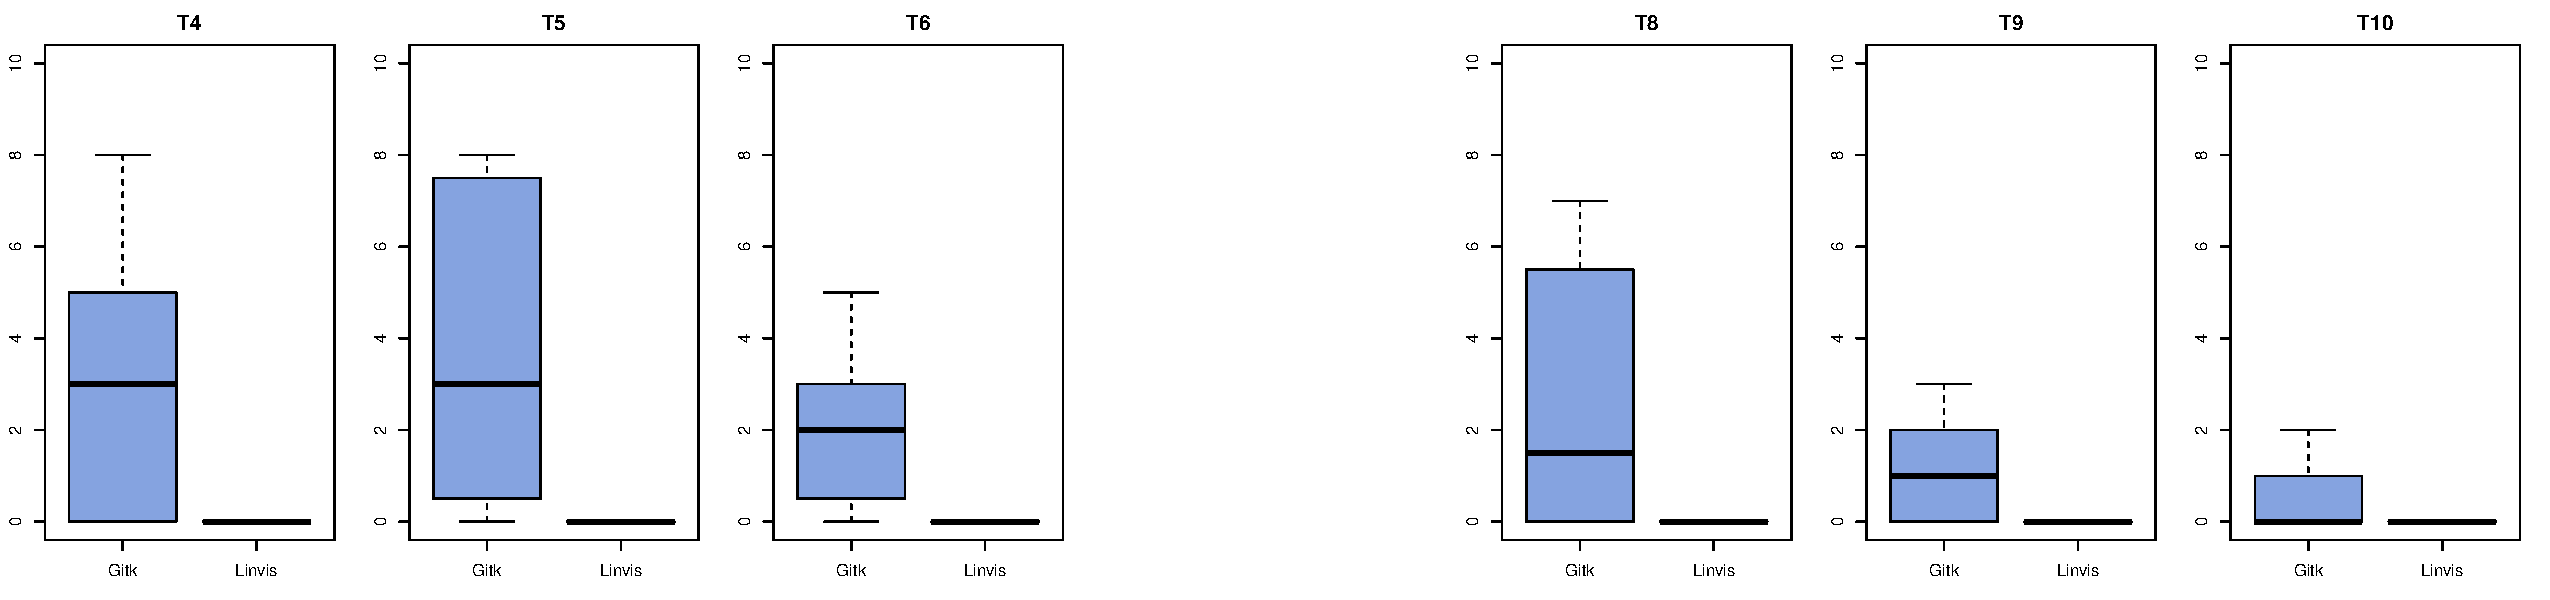
\includegraphics[width=0.9\linewidth]{Figures/evaluation/accuracy.pdf}
  \caption{Aggregated Accuracy of the summarization results}
  \label{fig:agg_accuracy}
\end{figure}

The results indicate that in all tasks except for task T7, who
contributed the most changes, merge size did not have a significant
impact on the \textbf{time} taken to respond. The results are presented
in Table~\ref{tab:cross_commit_timing}.

\begin{table}[htpb]
  \centering
  \caption{Effect of merge size on response time}
  \label{tab:cross_commit_timing}
  \begin{tabular}{crl}
    \toprule
    Task & $p$-value & Conclusion\\\midrule
    T4   & 0.99      & Do not reject $H_0$\\
    T5   & 0.90      & Do not reject $H_0$\\
    T6   & 0.92      & Do not reject $H_0$\\
    T7   & 0.01      & Reject $H_0$\\
    T8   & 0.99      & Do not reject $H_0$\\
    T9   & 0.70      & Do not reject $H_0$\\
    T10  & 0.77      & Do not reject $H_0$\\
    \bottomrule
  \end{tabular}
\end{table}

Inspecting the results from commit 7, depicted in
Figure~\ref{fig:task_7_time}, the primary difference stems from the time
used to respond when using \tool{}. Participants much longer to produce
a response for the larger merge while using \tool{} than they did for
the smaller merge. Comparing this with the timing results for task T8,
in Figure~\ref{fig:task_8_time} where participants took very little time
to respond for both merges. Participants took considerably less time
using \tool{} than they did with Gitk.

\begin{figure}[htpb]
  \centering
  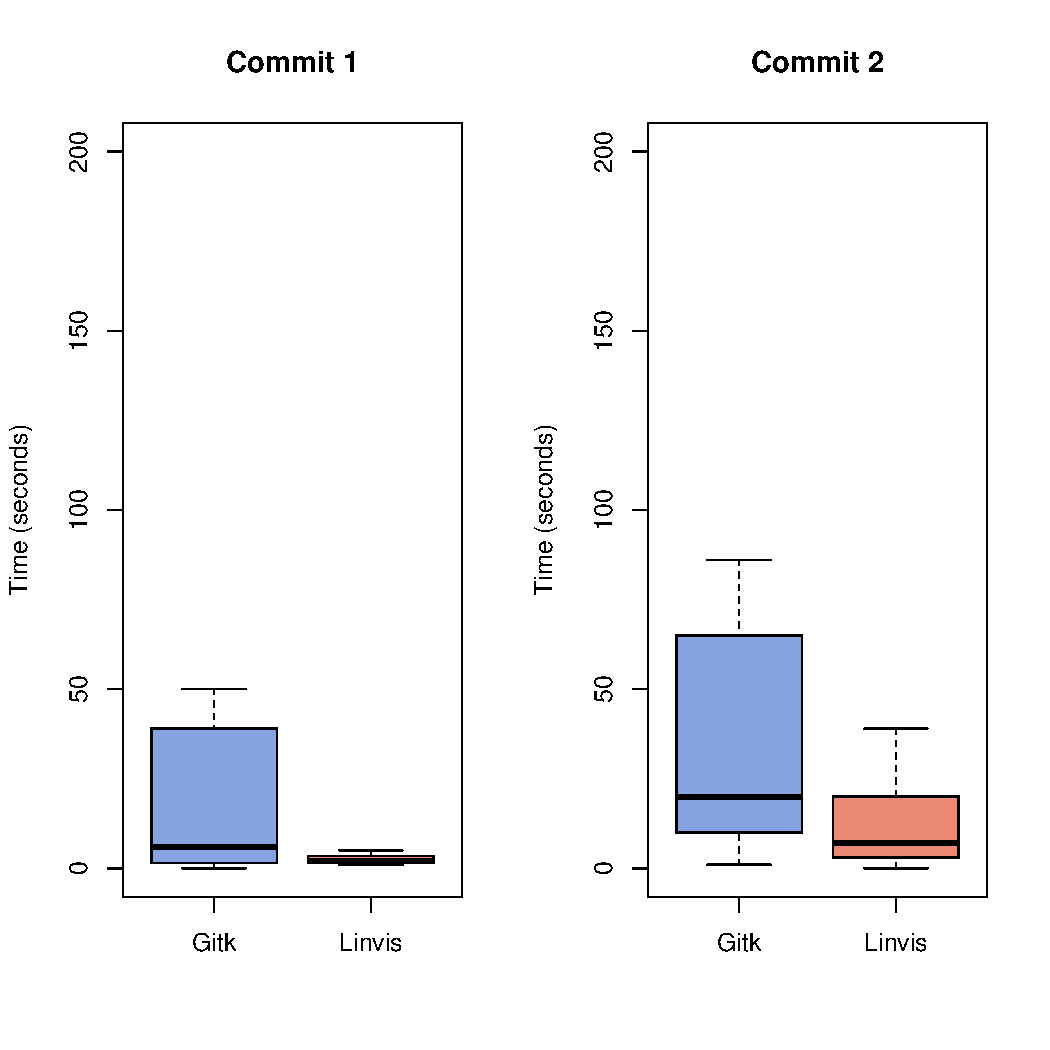
\includegraphics[width=0.5\linewidth]{Figures/evaluation/time/7.pdf}
  \caption{Difference in time taken to respond to task T7 between merge sizes}
  \label{fig:task_7_time}
\end{figure}

\begin{figure}[htpb]
  \centering
  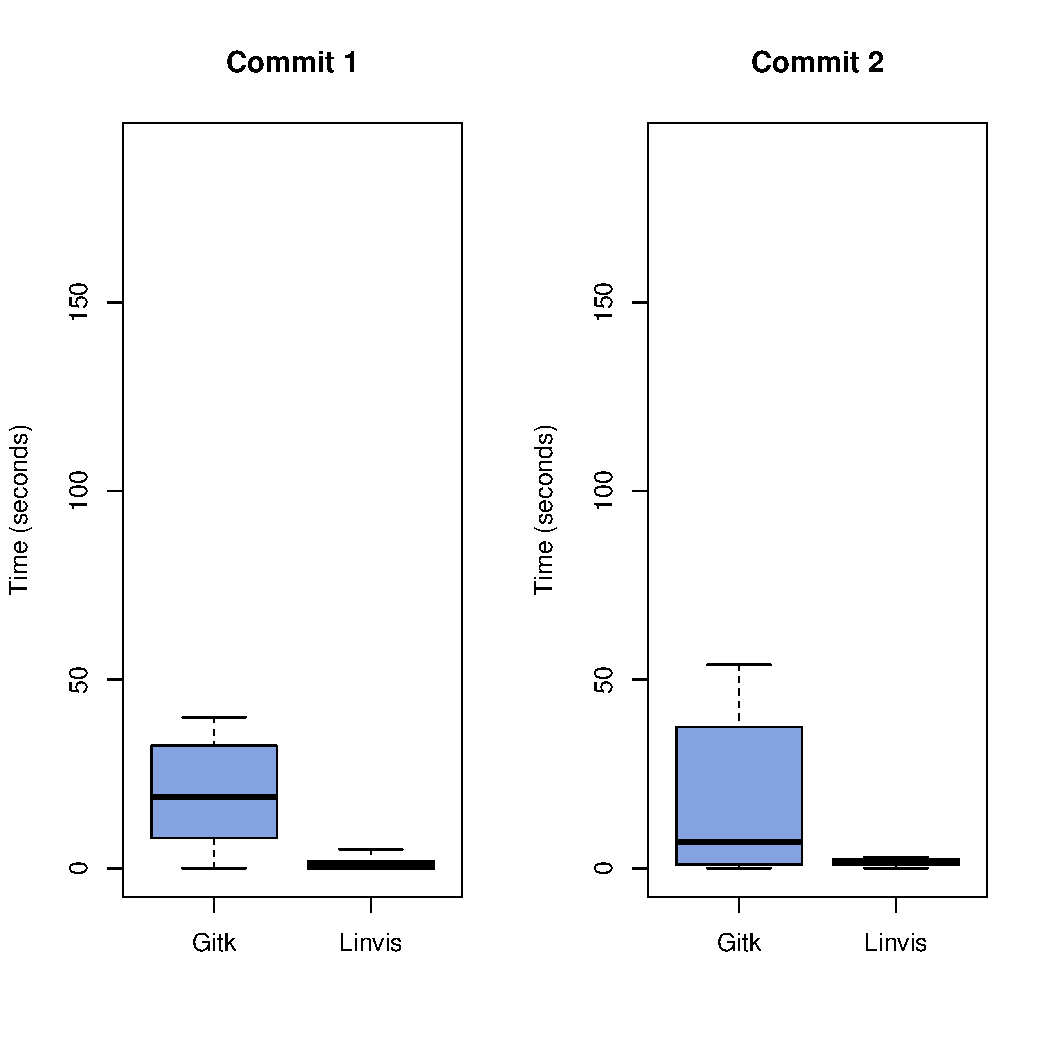
\includegraphics[width=0.5\linewidth]{Figures/evaluation/time/8.pdf}
  \caption{Difference in time taken to respond to task T8 between merge sizes}
  \label{fig:task_8_time}
\end{figure}

\begin{figure}[htpb]
  \centering
  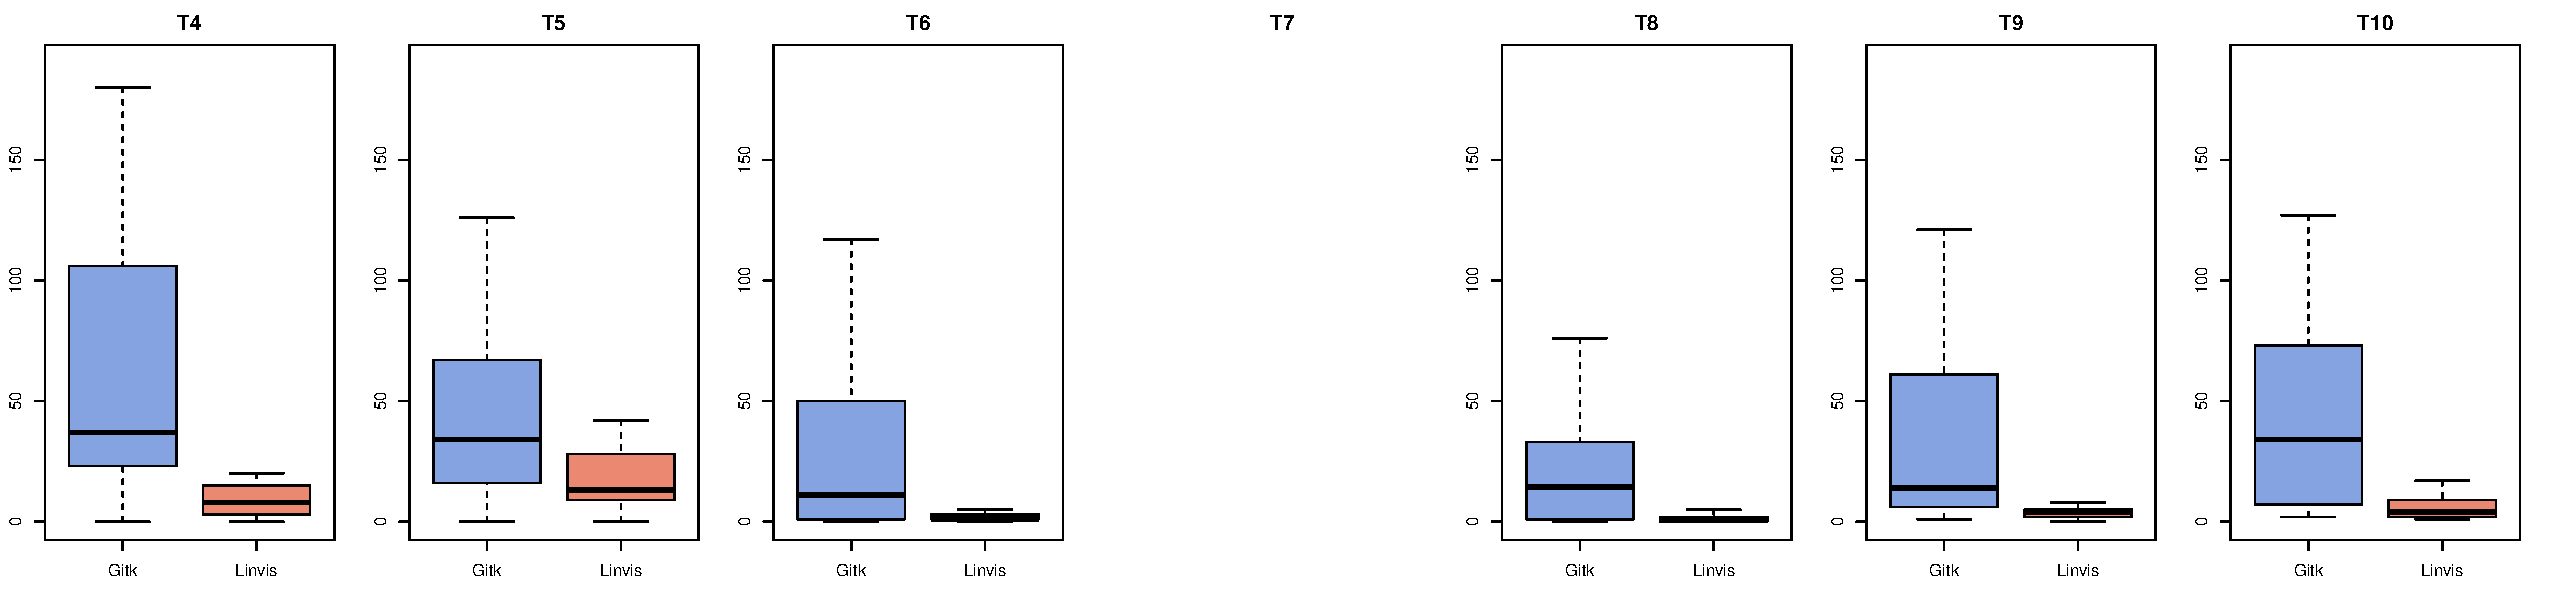
\includegraphics[width=0.9\linewidth]{Figures/evaluation/time.pdf}
  \caption{Aggregated Time to respond to summarization tasks}
  \label{fig:agg_time}
\end{figure}

The results do not indicate that there is a difference in the time taken
to respond between merge sizes for the other tasks. In all tasks, except
for T7, \tool{} does have a statistically significant impact on the time
taken to respond. \tool{} has a large impact on the time taken to
respond to tasks T4, T8, T9, and T10, determine the merges that led to
integration, the number of files modified, which files had the most
changes, and the modules involved. \tool{} had a medium effect on the
time taken to respond to tasks T5 and T6, what other commits are
integrated with this commit, and the other number of authored involved.
The direction of the effect is visible in Figure~\ref{fig:agg_time}.
Inspecting the results from task T7 in Figure~\ref{fig:task_7_time},
\tool{} appears to have an effect, and Cliff's delta indicates that in
the case of the medium-sized merge, that there is a medium effect. So
why does the Wilcoxon test indicate that the null hypothesis should not
be rejected? This is likely due to the sample size; the Wilcoxon test is
related to the sample size, while the delta effect size is not. Since
the results in task T7 are not aggregated, the number of samples is
effectively cut in half, from 22 down to 11, which is not enough to have
confidence that the results are representative of the population. The
effect size says that if our sample is representative of the population,
this is the impact that could be expected. The results of the tests are
presented in Table~\ref{tab:accuracy_results}.

\begin{table}[htpb]
  \centering
  \caption{Aggregated time results, including the Wilcoxon
    $p$-values and Cliff's Delta Effect size}
  \label{tab:accuracy_results}
  \begin{tabular}{clrcc}
    \toprule
    Task                & $p$-value & Delta Est. & Conclusion          & Effect\\\midrule
    T4                  & 0.0006    & 0.605      & Reject $H_0$        & Large\\
    T5                  & 0.0241    & 0.399      & Reject $H_0$        & Medium\\
    T6                  & 0.0254    & 0.388      & Reject $H_0$        & Medium\\
    \multirow{2}{*}{T7} & 0.2586    & 0.289      & Do not reject $H_0$ & Small\\
                        & 0.1146    & 0.405      & Do not reject $H_0$ & Medium\\
    T8                  & 0.0018    & 0.545      & Reject $H_0$        & Large\\
    T9                  & 0.0002    & 0.667      & Reject $H_0$        & Large\\
    T10                 & 0.0002    & 0.649      & Reject $H_0$        & Large\\
    \bottomrule
  \end{tabular}
\end{table}

To summarize, \tool{} is able to assist users determine the series of
merges a commit passes through to integration, the other commits
integrated with it, the number of authors, how many files were modified,
and which file had the most changes more quickly and accurately than
with Gitk. \tool{} does not have an impact on the accuracy when
determining the modules involved in the merge, but does have an impact
on the time taken to respond. \tool{} does not appear to have an impact
on the time take to determine who contributed the most changes, but does
have an impact on accuracy and correctness. Interestingly, there is a
medium effect on the time taken to respond in the case of the larger
merge, but little confidence in this effect. More participants are
required in order to determine if \tool{} makes a difference.

\subsection{User Opinions}
\label{sub:user_opinions_results}

Among the 12 participants, there was nearly unanimous agreement that for
conceptual understanding and summarization tasks, \tool{} was easier to
use than Gitk. The participants cited the ability to abstract
information about the merge from the clean summarization tables and
simple visualizations as the primary reasons for preferring \tool{} to
Gitk. Three participants suggested that someone with a professional
understanding of Gitk and the git command-line may be able to extract a
conceptual understanding from the DAG visualization and perform the
summarization tasks. One of these three participants said that they
would prefer to have both tools available, as they are able to
complement each other.
